\chapter{Methodik}

\section{Eyetracking}

In dieser Studie wurde die Methode des Eyetrackings benutzt, um die Augenbewegungen der \gls{PuP} auf dem Bildschirm festzuhalten. Im Folgenden werden kurz die Einrichtung und die Funktionsweise eines Eyetracking Monitors beschrieben. 

Geräte, welche Blickbewegungen aufzeichnen können, unterscheiden sich in zwei grundlegende Kategorien:
    \begin{itemize}
        \item Aufzeichnung über eine Brille erstellen
        \item Kamera unterhalb des Bildschirms verwenden
    \end{itemize}


Im folgenden Versuchsaufbau wurde die zweite Variante gewählt. Hierbei ist es essenziell, dass \gls{dPodP} auf der richtigen Höhe sitzt und einen ungehinderten Blick (keine Brille) auf den Bildschirm hat. Ebenso wichtig ist, dass \gls{dPodP} seinen Kopf ruhig hält und nur die Augen bewegt. Bei einer übermäßigen Bewegung des Kopfes würden die aufgezeichneten Daten verfälscht. Bevor mit der eigentlichen Studie begonnen werden kann, muss die Kamera kalibriert werden. Der Versuchsteilnehmer folgt einem Punkt auf dem Bildschirm, um die richtige Einstellung des Gerätes zu ermöglichen. 


Im Versuchsaufbau sitzt, wie in der Abbildung beschrieben, \gls{dPodP} (P) vor dem Bildschirm, der Versuchsleiter (V) auf der gegenüberliegenden Seite.
Die Kamera, welche die Blickbewegungen des Versuchsteilnehmers aufzeichnet, befindet sich unter dem Anzeigebildschirm. Dieser Aufbau wurde gewählt, damit \gls{dPodP} einfach \grqq weiter\grqq oder das Ergebnis einer Aufgabe sagen kann, ohne den Blick vom Anzeigebildschirm zu lösen. Auf die Verwendung einer Tastatur wurde verzichtet, weil mit jedem Blick darauf eine erneute Kalibrierung von Nöten wäre.

\begin{figure}[H]
\noindent\hspace{0.5mm}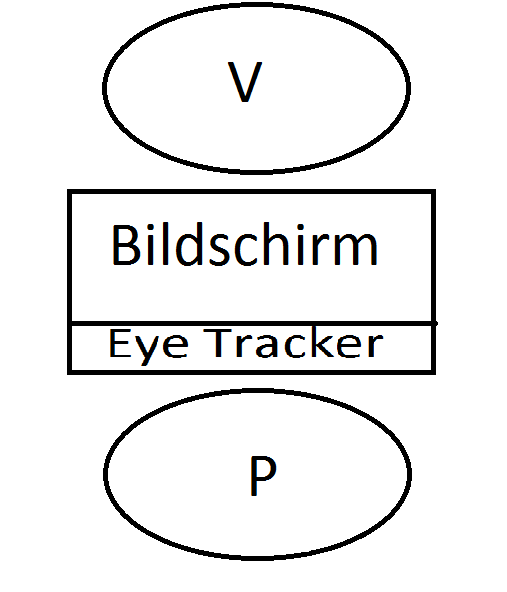
\includegraphics[width=8cm]{./Ressourcen/Versuchsaufbau.png}
\caption{Versuchsaufbau, Lorenz Müller}
\end{figure}

\section{Begriffserklärung und Instrumentenbeschreibung}
Im Folgenden werden notwendige Begriffe erklärt, sowie Angaben zur Datenauswertung ausgeführt.


Beginnend mit dem Begriff \grqq Fixationen auf ein bestimmtes Objekt \grqq ist in dieser Studie ein messbares Innehalten des Versuchsteilnehmers, auf einer bestimmten Stelle des Bildschirms gemeint. Laut der Diplomarbeit \citetitle{EyetrackingFixation} der Uni Stuttgart: \grqq (Beträgt) diese Zeitdauer ... typischerweise 100 bis 200ms.\grqq

Somit sind die Fixationen bei einer Auswertung von Eyetrackinguntersuchungen immer in drei Teile unterteilt:
    \begin{itemize}
        \item Die Koordinaten der einzelnen Fixation, meist aufgeteilt in einen x und einen y Wert.(Horizontal, Vertikal)
        \item Die Dauer der jeweiligen Fixation
        \item Die zeitliche Reihenfolge der Fixation
    \end{itemize}


Durch \textit{AOI}`s (\grqq Area of Interrest\grqq) kann der für den \gls{PuP} sichtbare Bereich des Bildschirms in Abschnitte unterteilt werden, welche für die Auswertung relevant sind. In vorliegender Studie wurden auf der ersten Seite AOIs über die Textabschnitte, sowie über die Graphiken gelegt, um die Fixationen auf diesem Bereich feststellen zu können. Ebenso wurde in den letzten Bereich eine AOI gelegt, um das Unterscheiden vom ersten zum zweiten Durchgang zu ermitteln (mehr dazu im Teil eigene Einteilung).

Eine \textit{Heatmap} ist eine Darstellung des Bildschirms, in der die Benutzerfixationen anhand von ihrer Häufigkeit und Dauer eingefärbt werden. Hierbei können Zonen, welche vom Benutzer intensiv betrachtet werden, schnell veranschaulicht werden.

Diese Daten wurden mit Hilfe des Eyetrackingapperates RED 500 festgehalten und konnten unter Verwendung des Programms IViewx unterteilt werden. Somit konnte die Anzahl der Fixationen in einem Bereich ausgewertet werden. Die Daten wurden verwendet, um die Gruppeneinteilung im folgenden Verlauf der Arbeit vorzunehmen.

Nach der Einteilung der Gruppen wurden zum einen Varianzanalysen zu den gegebenen Forschungsfragen angestellt. Die Auswertung erfolgte über eine einfaktorielle ANOVA um signifikante Unterschiede in den Gruppen oder unter den Bildern feststellen zu können. Zum anderen wurden die Mittelwerte berechnet und verglichen. Diese Auswertungen sind im Teil Ergebnis festgehalten.

\section{Ablauf der Studie}

Auf der ersten Folie wurde den Versuchsteilnehmern ein Teilbarkeitsbeweiß von drei oder fünf aufeinanderfolgender Zahlen, anhand eines heuristischen Lösungsbeispiels veranschaulicht. Hierbei wurde gezeigt, dass drei aufeinander folgende Zahlen z.B 3,4,5 in der Summe (in unserem Beispiel 12) wieder durch die Anzahl der aufeinander folgenden Zahlen mit ganzzahligem Ergebnis teilbar ist. Somit kann in unserem Beispiel die 12 durch 3 geteilt werden, ohne einen Rest zu erhalten.
Analog funktioniert es bei jeder ungeraden Anzahl an aufeinanderfolgenden natürlichen Zahlen. Die erste Folie unterteilt sich in Heuristiken, welche den allgemeinen Lösungsweg des Beweises aufzeigen soll und in Inhalt, welcher von textueller oder bildlicher Form sein kann. Die bildliche Form ist zum einen ein Anfangsbeispiel, bei dem die Hypothese bei unterschiedlichen Zahlen überprüft wird, zum anderen eine Möglichkeit, wie man durch Sortierung den Sachverhalt besser veranschaulichen kann. In textueller Form wurden die Überlegungen hierzu festgehalten.

Darauffolgend wurden den \gls{PuP} neun mathematische Aufgaben gestellt, welche sie mit Hilfe einer Multiple-Choice-Antwortmöglichkeit bearbeiten sollten. Beispiel einer Aufgabe:

\begin{figure}[H]
\noindent\hspace{0.5mm}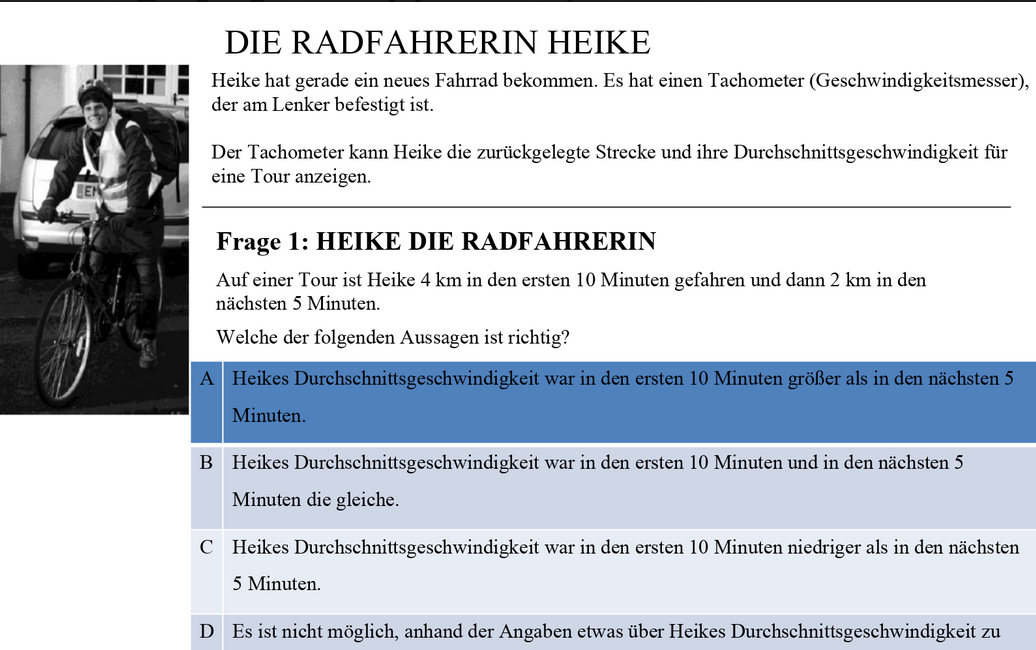
\includegraphics[width=15cm]{./Ressourcen/Radfahrerin.png}
\caption{Aufgabenstellung Radfahrerin, Lorenz Müller}
\end{figure}

\section{Aufgabe-Bildeinteilung}

Bilder und Graphiken wurden in der Studie wie folgt unterteilt:

Die ersten beiden Aufgabestellungen \gls{Rad} handeln von einer Radfahrerin, wobei lediglich ein Bild dieser zusehen ist. Es trägt nicht zur Veranschaulichung oder Unterstützung der Versuchsperson bei und ist somit als dekorativ zu bezeichnen. 


In der nächsten Aufgabenstellung \gls{Ren} ist ein Graph über die Geschwindigkeit eines  Rennfahrers in Abhängigkeit vom Weg zu sehen. Dieser muss verwendet werden, um die Aufgabenstellung zu bearbeiten, das Bild ist somit essenziell. 


In der darauffolgenden geschilderten Problematik \gls{Zuf} werden zwei Graphiken, welche Teile eines Zufallsexperiments darstellen, verwendet. Hierbei müssen die Felder des Glücksrades und die Verteilung der Kugeln betrachtet werden, um die Aufgabenstellung lösen zu können. Somit sind die Graphiken ebenso essenziell.


Die nächsten beiden Aufgaben handeln vom Bergsteigen \gls{Ber}. Hierbei ist lediglich ein Berg als Bild gegeben, welcher aber für die Bearbeitung der Aufgabe nicht nützlich ist. Auch dieses Bild hat damit einen dekorativen Zweck.


Im Anschluss wird noch eine Aufgabe im Themenbereich des Autofahrens gegeben \gls{Aut}. Dabei wurde wiederum ein Graph verwendet, der die Geschwindigkeit und die Zeit der Autofahrerin in Relation setzt. Diese Graphik ist essenziell für die Bearbeitung der Aufgabe. 


In den letzten beiden Aufgabestellungen wurde sowohl eine Tabelle, welche essenziell für die Bearbeitung ist, als auch ein einfaches Bild von einem Auto, welches eher dekorativen Charakter hat, verwendet. Da hierbei eine Mischung von Bildtypen verwendet wurde, werden diese beiden Aufgaben in der weiteren Bearbeitung nicht weiter betrachtet. 

Somit kommen in dieser Bildzuweisung lediglich drei essenzielle, vier dekorative Bilder und keine repräsentativen Bilder vor. Dabei sollte der Unterschied zwischen hilfreichen und nicht hilfreichen Bildern besser erkennbar sein.


\section{Gruppeneinteilung}

Aus den oben genannten Lerntypen wurden drei Gruppierungen gebildet: \gls{Gr1} der Unsichere, \gls{Gr2} der Problemlöser, \gls{Gr3} der Textuelle. Mit den gesamt 39 \gls{PuP} wurde versucht, eine sinnvolle Unterteilung zu treffen. Wie in der Tabelle (Ausprägungen) zu sehen ist, wurde die Verbindung unterschiedlicher Ausprägungen genutzt. Bei 22 Versuchsteilnehmer konnte dies relativ eindeutig erfolgen. Bei den restlichen 17 war dies aufgrund von sich widersprechenden Einzelfaktoren für die Zuweisung nicht möglich. Weitere Typologien wären dennoch möglich, wurden in dieser Studie aus Gründen der Systematik nicht weiter verfolgt.

Das erstmalige Lesen des Textes dauerte im Schnitt über alle \gls{PuP} hinweg 110,4 Sekunden. Diese Dauer konnte ermittelt werden, indem in einer AOI am Ende des Textes Fixationen festgestellt wurden. Sobald also ein Versuchsteilnehmer in dieses Feld geblickt hat, ist der erste Durchgang des Lesevorgangs beendet und der Zweite, welcher andauert, bis \gls{dPodP} auf die nächste Folie wechselt, folgt. Diese Einteilung konnte anhand von Messungen der Zeit und der Reihenfolge der Fixationen belegt werden. 


Die \gls{PuP} wiesen im Durchschnitt folgende Werte auf:
    \begin{itemize}
        \item Dauer des Zweiten Durchgangs: 72,6 Sekunden 
        \item Fixationen auf die Bildbereiche im zweiten Durchgang: 75,2
        \item Fixationen auf die Textbereiche im zweiten Durchgang: 71,1
    \end{itemize}

Die Versuchsteilnehmer wurden auf die genannten Merkmale untersucht und in die passenden Gruppen anhand dieser Einteilung zugeordnet.
\section*{Einteilungsschema}

\begin{table}[H]
\hspace{-5pt}
\begin{tabularx}{\textwidth + 5pt}{| @{\hspace{3pt}} M || @{\hspace{3pt}} M  | @{\hspace{3pt}} M  | @{\hspace{3pt}} M |}
\hline
\textbf{Ausprägungen} & \textbf{Typ Unsicher (Gr1.)} & \textbf{Typ Problemlöser (Gr2.)} & \textbf{Typ Textuell (Gr3.)}\\
\hline
\hline
Dauer 1. Durchgang          & (+) & 0 & 0\\
\hline
Dauer 2. Durchgang          & ++ & 0 & (+)\\
\hline
Textfixationen 2. Durchgang & + & 0 & +\\
\hline
Bildfixationen 2. Durchgang & + & + & 0\\
\hline
\end{tabularx}
\caption{Ausprägungen der Lerntypen}
\end{table}



\section{Schwierigkeiten bei der Erfassung}

Bei der Erfassung der Punkte einer Aufgabe wurde im Falle der richtigen Lösung lediglich ein Punkt vergeben. Kein Punkt wurde vergeben, wenn die Lösung falsch war. Es werden keine Teilpunkte vergeben. Falls ein Versuchsteilnehmer die Aufgabe in Teilbereichen richtig löste, anschließend aber dennoch im Ergebnis falsch lag, erhielt er dennoch 0 Punkte. Es findet somit eine Ergebnisorientierte- und keine Lösungswegorientierte Auswertung der Aufgaben statt, welche die Fähigkeiten der \gls{PuP} negativer abbildet als sie eigentlich sind.

Zusätzlich wurden Multiple-Choice-Antwortmöglichkeiten gegeben. Diese Methode erzeugt ebenso eine Unschärfe in der Lösung der Probandin oder des Probanden. Eine Verbesserung der Leistung des Versuchsteilnehmers wird durch die vierfache Antwortmöglichkeit der Aufgaben gegeben, da \gls{dPodP} durch Raten der richtigen Lösung mit einer Wahrscheinlichkeit von 1/4 oder 25 Prozent richtig liegt. Dies hat zur Folge, dass die Fähigkeiten der \gls{PuP} besser abgebildet werden als sie eigentlich sind.  

Ebenso war es für die \gls{PuP} nicht möglich, sich Aufgabenteile zu markieren oder sich nebenbei Notizen und Rechnungen auf Papier zu notieren. Dies hätte Kalibrierungsprobleme des Eye Tracking Automaten hervorrufen können. Dadurch wäre auch denkbar, dass sich dies negativ auf das Ergebnis auswirken könnte. Jedoch haben \citeauthor{schukajlow2011selbstberichtete} (\citedate{schukajlow2011selbstberichtete}) gezeigt, dass \grqq (b)ezüglich der selbstberichteten Strategienutzung und der mathematischen Modellierungsleistungen der Lernenden ... keine signifikanten Korrelationen festgestellt werden (konnten).\grqq Somit kann dieser Punkt nicht mit Sicherheit als negative Auswirkung für den \gls{PuP} gewertet werden. 

Die Einschränkungen der Ergebnisauswahl und des ergebnisorientierten Auswertungsansatzes wurden so gewählt, weil sie das Ergebnis der Studie schneller darstellbar machen. Im besten Fall könnten sich auch beide Effekte aufheben.
\section{Forschungsfrage}

Die Texte werden von den Versuchsteilnehmern unterschiedlich bearbeitet. Hierbei liegen unterschiedliche Teilbereiche in textueller oder in bildlicher Form im Fokus. Häufig ist das Lesen beim ersten Durchgang ein relativ linearer Vorgang, in dem von links nach rechts und weiter von oben nach unten gelesen wird. Nach dem ersten Durchgang unterscheiden sich die Probanden in dem sie einzelne Teilbereiche des Textes einer weiteren Betrachtung unterziehen. Dies führt uns zu der Frage:
(1) Kann man die \gls{PuP} anhand ihrer Augenbewegungen in Gruppen unterteilen und (2) kann die Unterteilung Aufschlüsse bezüglich der Leistungsfähigkeit innerhalb der Gruppe geben?

Ein weitere Teil der Studie besteht darin, das Ergebnis von \citeauthor{bockmannvalue} (\citedate{bockmannvalue}) in unserer Studie zu verifizieren (3), indem die unterteilten Aufgaben und die Gesamtpunktzahl der jeweiligen Aufgabe betrachtet wird. Somit wird untersucht ob ein direkter Zusammenhang im Lösen der Aufgabe und der Typologie des verwendeten Bildes besteht. Zuletzt wird noch untersucht, ob bestimmte Aufgabentypen für einzelne Probandengruppen positive oder auch negative Auswirkungen haben (4).